\documentclass{beamer}

\usepackage[italian]{babel}
\usepackage[utf8]{inputenc}

\usepackage{graphicx} % Immagini fantastiche e...
\graphicspath{        % dove trovarle
  {./images/},
  %{../images/}        % Necessario se cartella chapters
}

%\usepackage{float}
%\usepackage{color}
%\usepackage{caption}
%\usepackage{subcaption}

%\usepackage{hyperref}
%\hypersetup{colorlinks=true, linkcolor=black, citecolor=black, plainpages=false, urlcolor=blue}
\usepackage{wallpaper}
%\usepackage{algpseudocode,algorithm,algorithmicx}
%\usepackage{amssymb}
%\usepackage{amsmath}
%\usepackage{lipsum} 

\usepackage{algpseudocode,algorithm,algorithmicx}

 
% ================================ %
%          Cose Personali          %
% ================================ %
\newcommand\E{\ensuremath{\mathbb{E}}}
\newcommand\T{\ensuremath{\mathbb{T}}}
\renewcommand\inf{\ensuremath{\infty}}




%%Information to be included in the title page:
\title{Approfondimento di Intelligenza Artificiale}
\author{Tristano Munini}
%\institute{Overleaf}
  %\LARGE{\underline{\textbf{ANNO ACCADEMICO 2019-2020}}}\\
%\logo{
\includegraphics{polloPallido}}



% ================================ %
%            Il Documento          %
% ================================ %
\begin{document}

{
  \usebackgroundtemplate{
    \centering
    
\includegraphics[width=\paperwidth]{polloPallido}
  }
  \frame{\titlepage}
}

\begin{frame}
\frametitle{Indice}
\begin{itemize}
  \item AutoEncoders (AE) e Variational AutoEncoders (VAE)
  \item Generative Adversarial Network (GAN)
  \item Reinforcement Learning (RL)
    \begin{itemize}
      \item QNN
      \item Policy Gradient
    \end{itemize}
  \item GAN + RL per generazione di testi
    \begin{itemize}
      \item SeqGAN
      \item LeakGAN
    \end{itemize}
\end{itemize}
\end{frame}

%\begin{frame}
%\frametitle{Introduzione}
%TODO
%\end{frame}

%\begin{frame}
%\frametitle{Riferimenti Esterni}
%cfr. MIT intro to deep learning
%\end{frame}

%%%%%%%%%%%%%%%%%%%%%%%%%%%%%%%%%%%%%%%%%%%%%%%%%%%%%%%%%%%%%%%%%%%%%%%%%%%%%%%%%%%%%%%%%%%%%%%%%%%
% AE and VAE
%%%%%%%%%%%%%%%%%%%%%%%%%%%%%%%%%%%%%%%%%%%%%%%%%%%%%%%%%%%%%%%%%%%%%%%%%%%%%%%%%%%%%%%%%%%%%%%%%%%
\begin{frame}
\frametitle{AutoEncoders}
$ x \in \textrm{real data space}$
\\
$ z \in \textrm{latent space}$
\\
$ \hat x \in \textrm{real data space}$


\begin{figure}[ht]
  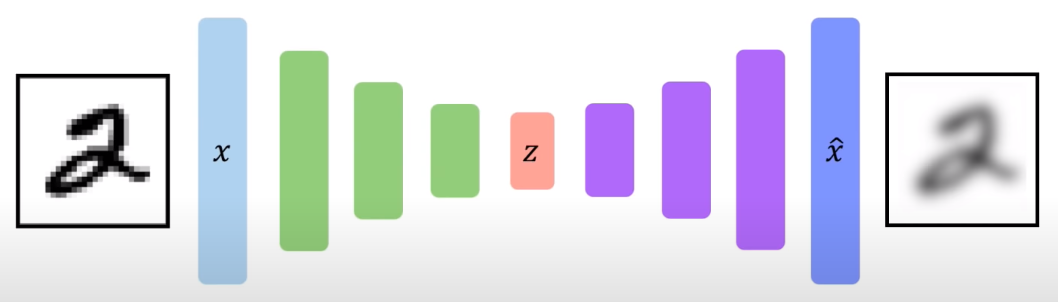
\includegraphics[width=\textwidth]{AE_01.png}
\end{figure}

The point of maximum compression, where $z$ is produced, is called bottleneck of the network

\end{frame}

\begin{frame}
\frametitle{Variational AutoEncoders}
$z$ is sampled from  the distribution with mean vector $\mu$ and standard deviation vector $\sigma$.
\\
We want an $\hat x$ that is similar to $x$ but that has some differences.
We want a variation of $x$.
\begin{figure}[ht]
  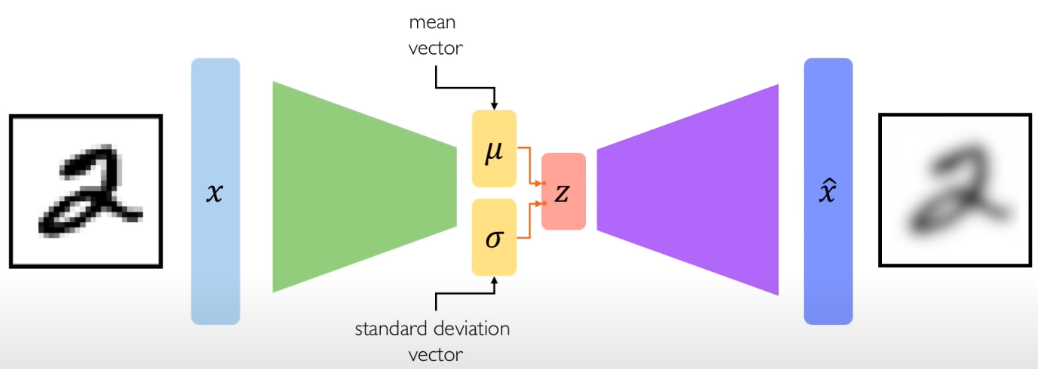
\includegraphics[width=\textwidth]{VAE.png}
\end{figure}
\end{frame}

\begin{frame}
\frametitle{Reparametrization Trick}
We can not use $z \sim \mathcal{N}(\mu, \sigma ^ 2)$
\\
So we use
\begin{align*}
  z = \mu + \sigma \odot \varepsilon
  \quad \textrm{where $\varepsilon  \sim \mathcal{N}(0,1)$}
\end{align*}
Where $\odot$ notes the element-wise multiplication
\\
Now $z$ is the sum of two fixed vectors, $\mu$ and $\sigma$, and a random constant $\varepsilon$ used as a weight

%\begin{figure}[ht]
%  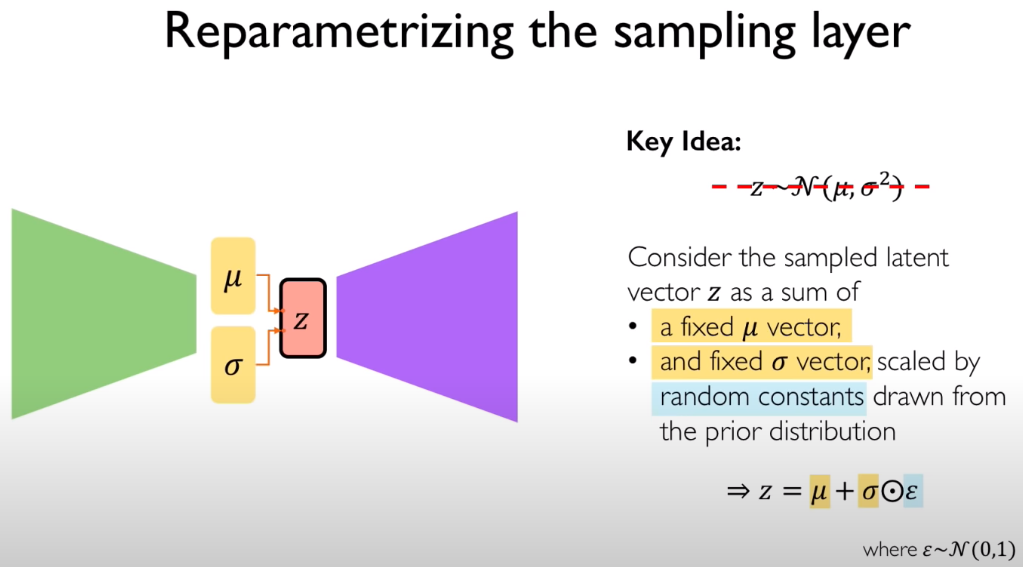
\includegraphics[width=\textwidth]{VAE_reparam_trick.png}
%\end{figure}
\end{frame}

\begin{frame}
\frametitle{Reparametrization Trick}
\begin{figure}[ht]
  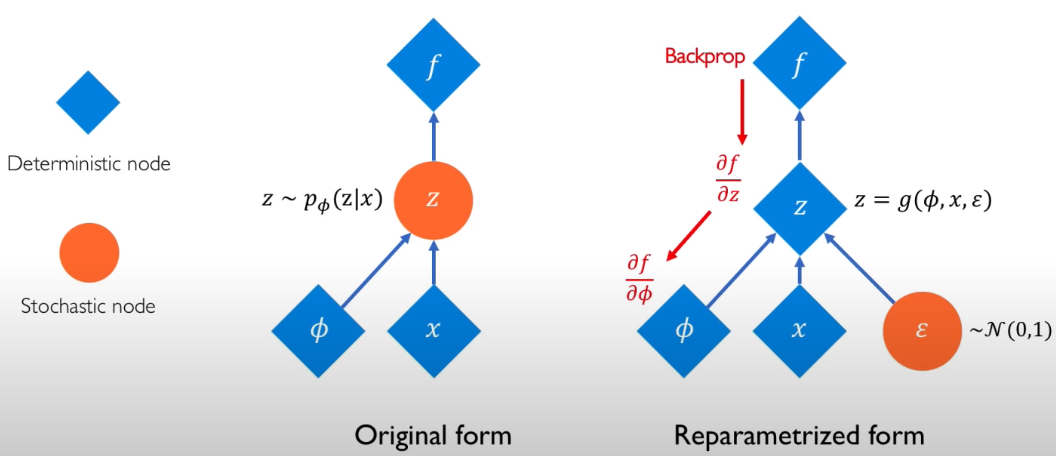
\includegraphics[width=\textwidth]{VAE_reparam_trick_backprop_01.png}
\end{figure}
\end{frame}

%%%%%%%%%%%%%%%%%%%%%%%%%%%%%%%%%%%%%%%%%%%%%%%%%%%%%%%%%%%%%%%%%%%%%%%%%%%%%%%%%%%%%%%%%%%%%%%%%%%
% GAN
%%%%%%%%%%%%%%%%%%%%%%%%%%%%%%%%%%%%%%%%%%%%%%%%%%%%%%%%%%%%%%%%%%%%%%%%%%%%%%%%%%%%%%%%%%%%%%%%%%%
\begin{frame}
\frametitle{Generative Adversarial Networks}
GANs are a way to make a generative model by having two neural networks compete with each other
\begin{figure}[ht]
  %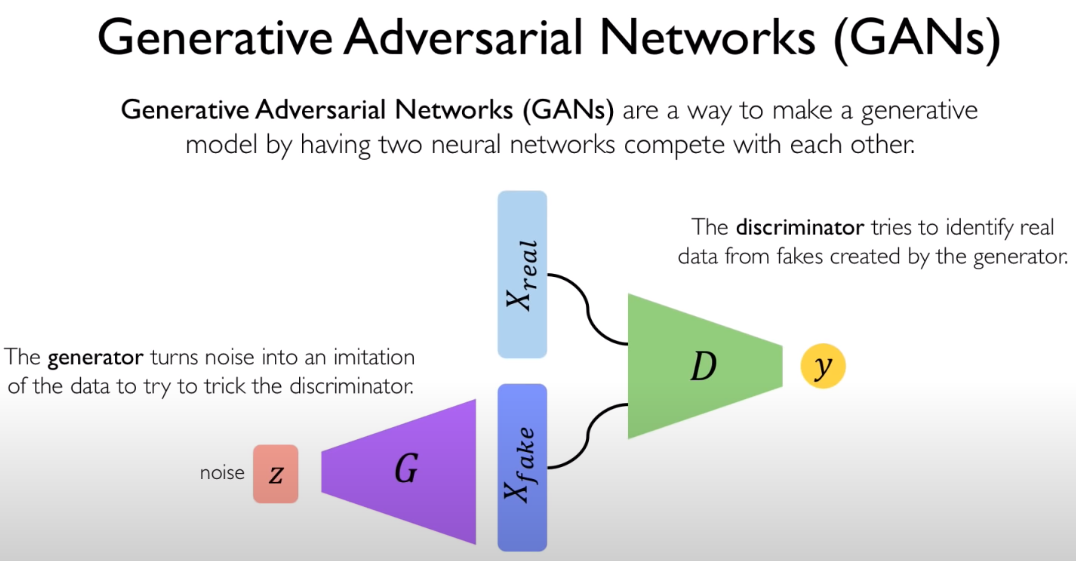
\includegraphics[width=\textwidth]{GAN.png}
  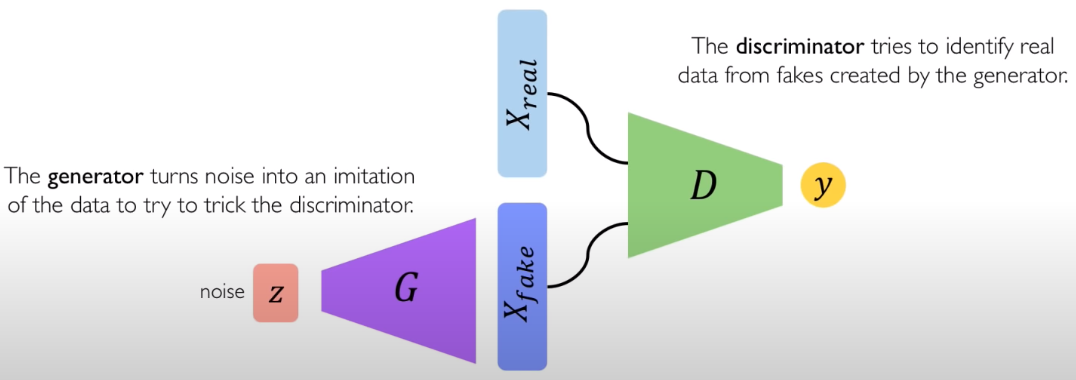
\includegraphics[width=\textwidth]{GAN_01.png}
\end{figure}
$z$ can be sampled form $\mathcal{N}(0,1)$ as in the VAEs
\end{frame}

\begin{frame}
\frametitle{GAN Training}
It is a min-max game
\begin{align*}
  min_G \, max_D \: V(D,G) &=
    \E_{x \sim P_{real(x)}} [ log D(x) ]
    \\                     &+
    \E_{z \sim P_z(x)} [ log ( 1 - D(G(z)) ]
\end{align*}
Where $P_{real(x)}$ is the probability distribution of the real data and $P_z(x) = \mathcal{N}(0,1)$ in our case

\end{frame}

\begin{frame}
\frametitle{GAN Problems}
\begin{itemize}
  \item Hard to converge to a good solution
  \item Vanishing gradient problem
  \item Model collapse
  \item Hard to find equilibrium
\end{itemize}
\end{frame}



%%%%%%%%%%%%%%%%%%%%%%%%%%%%%%%%%%%%%%%%%%%%%%%%%%%%%%%%%%%%%%%%%%%%%%%%%%%%%%%%%%%%%%%%%%%%%%%%%%%
% RL
%%%%%%%%%%%%%%%%%%%%%%%%%%%%%%%%%%%%%%%%%%%%%%%%%%%%%%%%%%%%%%%%%%%%%%%%%%%%%%%%%%%%%%%%%%%%%%%%%%%
\begin{frame}
\frametitle{Reinforcement Learning}
\begin{figure}[ht]
  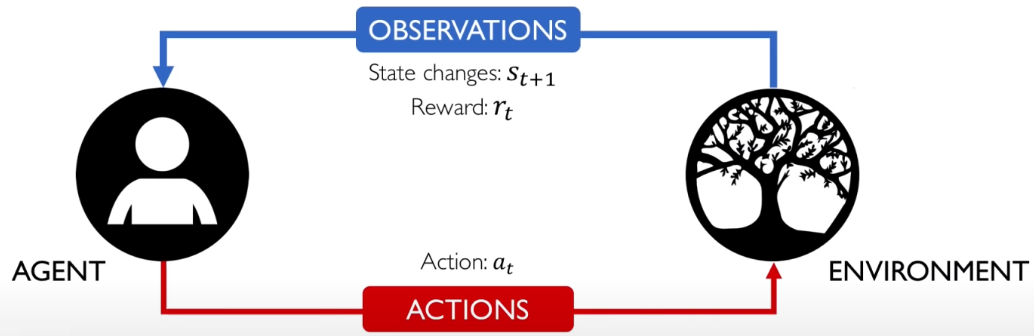
\includegraphics[width=\textwidth]{RL_schema.png}
\end{figure}

\textrm{Total Reward (Return)}
$$
\quad R_t = \sum_{i=t}^{\inf} r_i = r_t + r_{t+1} + \dots + r_{t+n} + \dots
$$
\textrm{Discounted Total Reward (Return)}
$$
\quad R_t = \sum_{i=t}^{\inf} \gamma^i r_i = \gamma^t r_t + \gamma^{t+1} r_{t+1} + \dots + \gamma^{t+n} r_{t+n} + \dots
$$

%\begin{figure}[ht]
%  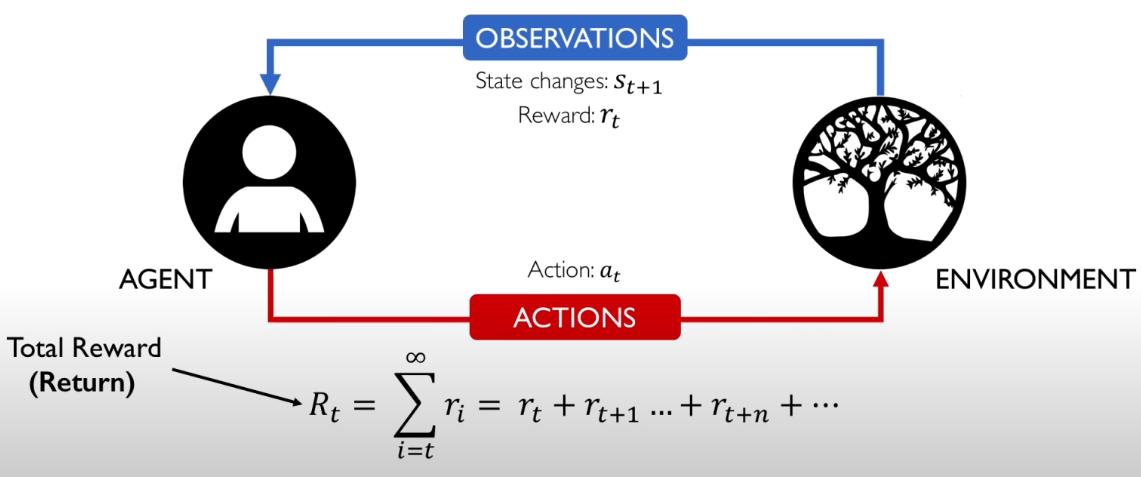
\includegraphics[width=\textwidth]{RL_key_concept.png}
%  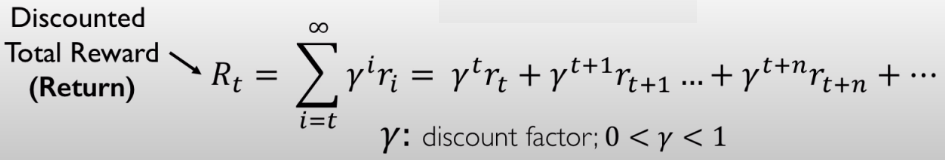
\includegraphics[width=\textwidth]{Discounted_Total_Reward.png}
%\end{figure}
\end{frame}

\begin{frame}
\frametitle{Quality Function}
%$$
%R_t = r_t + \gamma r_{t+1} + \gamma^{2} r_{t+2} + \dots
%$$
The quality function, also called Q-function, is the expected total future reward an agent in state $s_t$ can receive by doing action $a_t$
$$
Q(s_t, a_t) = \E [ R_t | s_t, a_t]
$$
\\
The policy that the agent follows is
$$
\pi (s_t) = argmax_a Q(s_t, a)
$$

%\begin{figure}[ht]
%  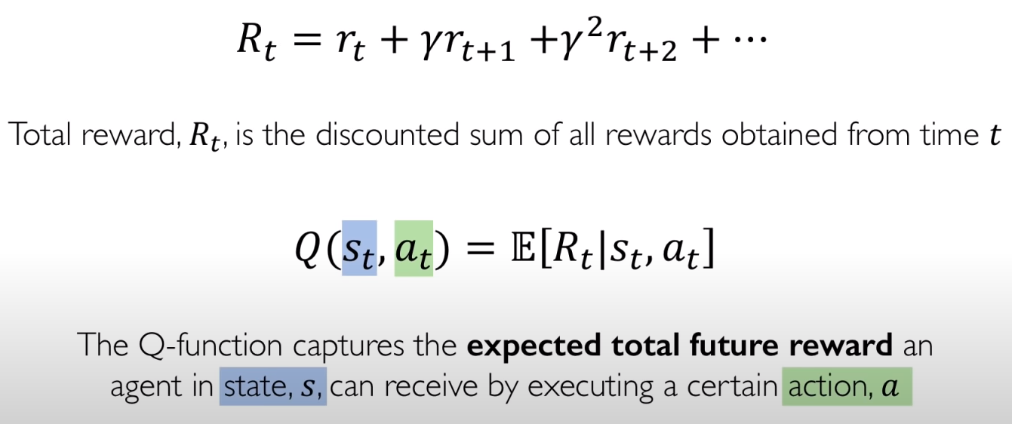
\includegraphics[width=\textwidth]{Q-Function.png}
%  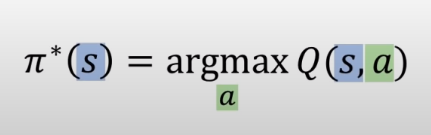
\includegraphics[width=.5\textwidth]{Policy_Fun.png}
%\end{figure}
\end{frame}


%\begin{frame}
%\frametitle{template}
%\begin{figure}[ht]
%  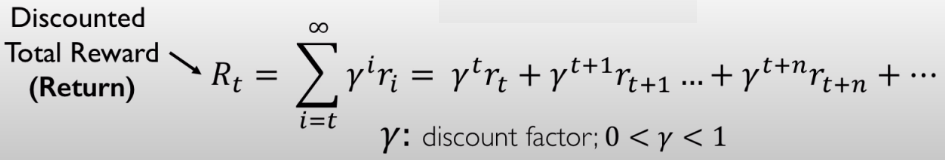
\includegraphics[width=\textwidth]{Discounted_Total_Reward.png}
%  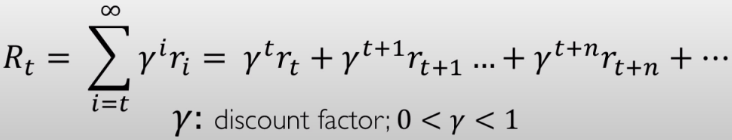
\includegraphics[width=\textwidth]{Discounted_Total_Reward_Formula.png}
%\end{figure}
%\end{frame}

\begin{frame}
\frametitle{QNN}
It may be hard to find manually a good Q-Function
\\
We can use an NN to estimate $Q(s_t, a)$ for all possible actions $a$
\begin{figure}[ht]
  %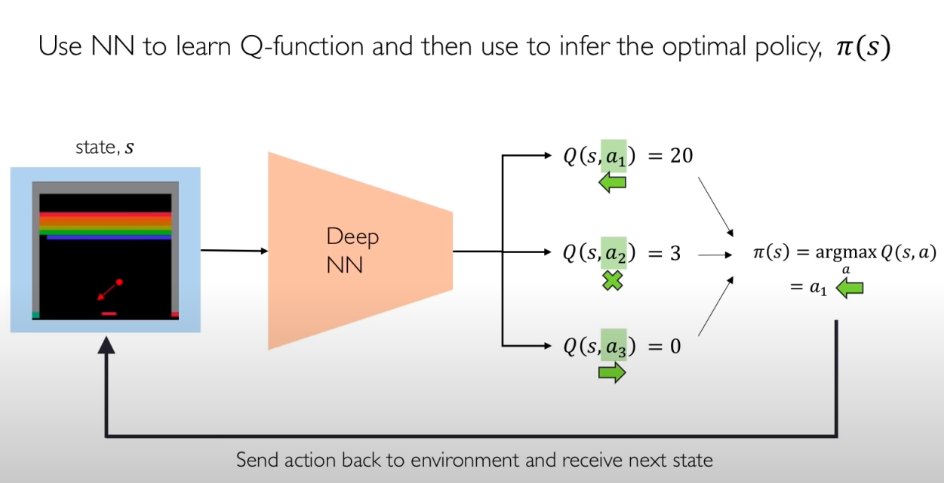
\includegraphics[width=\textwidth]{QNN.png}
  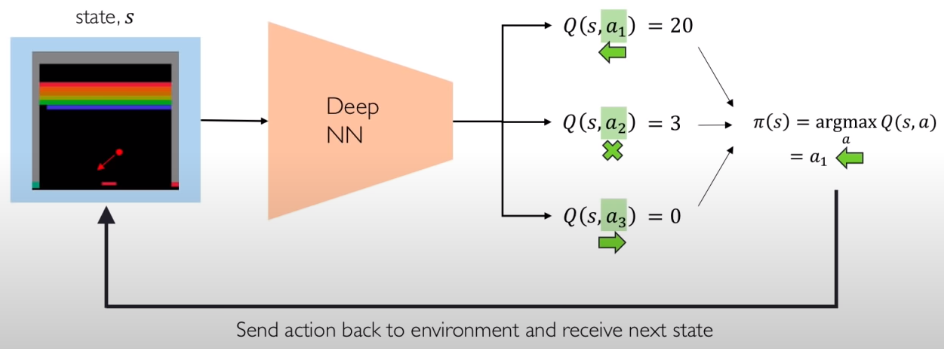
\includegraphics[width=\textwidth]{QNN_01.png}
\end{figure}
This solution is limited to discrete action space
\end{frame}

\begin{frame}
\frametitle{Policy Gradient}
What if we need to use an agent within a continuous action space?
\begin{figure}[ht]
  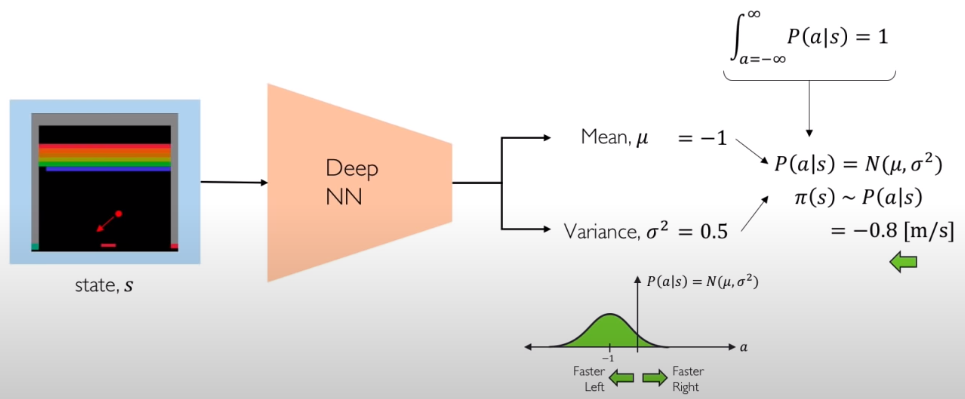
\includegraphics[width=\textwidth]{Pol_Grad.png}
\end{figure}
\end{frame}

\begin{frame}
\frametitle{Policy Gradient}
The loss used in Policy Gradient is
$$
loss = - logP(a_t| s_t) R_t
$$
so we weight the expected return (total reward in the future) with the probability of taking the action that gives this specific return
\\
\vspace{1cm}
Remember that the network chooses the next action using $\pi (s) \sim P(a|s)$
\end{frame}

\begin{frame}
\frametitle{N-Monte Carlo Rollouts}
$$
loss = - logP(a_t| s_t) R_t
$$
$R_t$ is a sum over infinity so we need to approximate it
\\
To do so we can use the Monte Carlo Rollouts:
\begin{itemize}
  \item use the current policy on current state $\pi(s_t)$ to calculate $N$ possible outcomes to state $s_{t+n}$ in the future
  \item sum all the $N$ rewards $r_i^k$ where $i=t, \dots, t+n$ and $k = 1, \dots, N$
  \item divide by $N$, so get the mean of the expected future reward from state $s_t$ with action $a_t$
\end{itemize}
\end{frame}

\begin{frame}
\frametitle{REINFORCE}
The REINFORCE Algorithm:
\begin{enumerate}
  \item from current state $s_t$ execute several times $\pi(s_t)$ until termination or state $s_{t+n}$
  \item calculate the mean of the expected future reward
  \item use the just calculated $R_t$ in the loss, and update the network
  \item sample an $a_t$ from the resulting distribution $\pi(s_t)$, and repeat from 1
\end{enumerate}
Notice that step 1 and 4 are an explore and exploit step, respectively
\end{frame}


%%%%%%%%%%%%%%%%%%%%%%%%%%%%%%%%%%%%%%%%%%%%%%%%%%%%%%%%%%%%%%%%%%%%%%%%%%%%%%%%%%%%%%%%%%%%%%%%%%%
% GAN + RL for text
%%%%%%%%%%%%%%%%%%%%%%%%%%%%%%%%%%%%%%%%%%%%%%%%%%%%%%%%%%%%%%%%%%%%%%%%%%%%%%%%%%%%%%%%%%%%%%%%%%%
\begin{frame}
\frametitle{GAN + RL for text}
We want to generate long sequences of words (tokens) that resemble human generated sentences
\\
To tackle this difficult problem we use an RNN-based GAN architecture with an RL approach for the Generator
\\
\vspace{0.5cm}
The SeqGAN are the first kind of network presented and can generate sequences up to 20 tokens
\\
\vspace{0.5cm}
The LeakGAN are based on the previous but are more robust and can generate really good results with sentences of 40 words
\end{frame}

\begin{frame}
\frametitle{SeqGAN}
The Sequential GAN architecture
\begin{figure}[ht]
  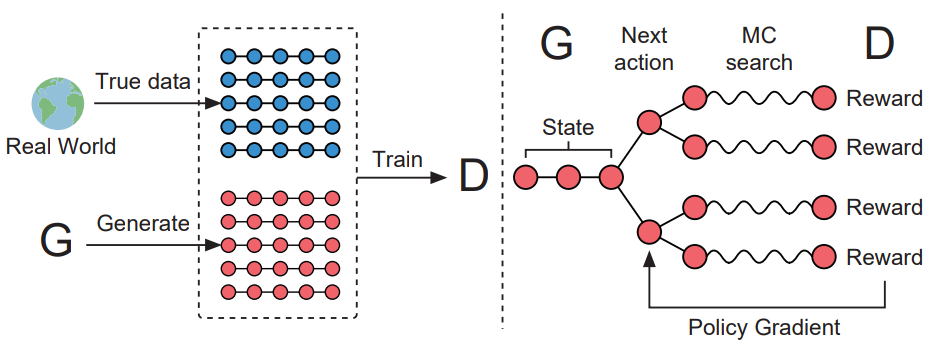
\includegraphics[width=\textwidth]{SeqGAN_Idea.png}
\end{figure}
\end{frame}

\begin{frame}
\frametitle{SeqGAN}
The schema of the RNN used inside the Generator of a SeqGAN
\begin{figure}[ht]
  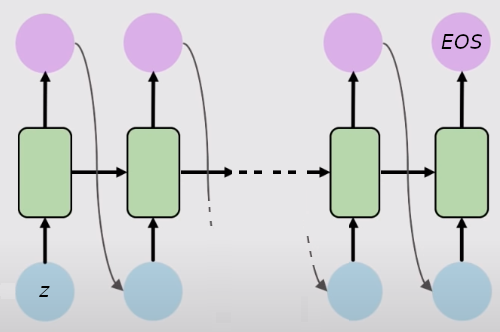
\includegraphics[width=.6\textwidth]{RNN_01.png}
  %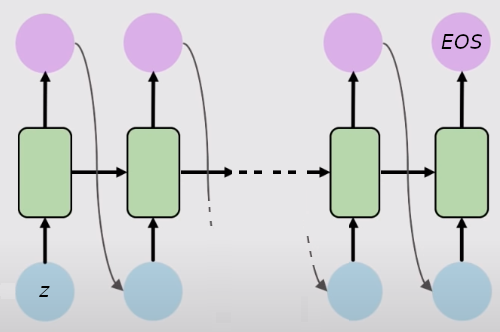
\includegraphics[height=.4\textheight]{RNN_01.png}
\end{figure}
The first blue dot is a noise $z$ and the last pink dot is a special ``End Of Sequence'' token 
\\
In the case of SeqGAN EOS is generated after 20 tokens
\end{frame}

\begin{frame}
\frametitle{Loss Function for G}
$$
J(\theta) = \E[R_t | s_0, \theta ] =
\sum_{y_1 \in \T}
G_\theta ( y_1 | s_0) \cdot
Q_{D_\phi}^{G_\theta} ( s_0, y_1)
$$
where $G_\theta$ is the generator with parameters $\theta$ and $ Q_{D_\phi}^{G_\theta} (s, a) $
is the future reward gained by doing action $a$ in state $s$ following the policy given by $G_\theta$
\\
Note that $\T$ is the action space composed by all the legal tokens (words) and $s_0$ is the noise vector $z$
\end{frame}

\begin{frame}
\frametitle{Loss Function for G}
We need to estimate $ Q_{D_\phi}^{G_\theta} ( s_{t-1}, y_t) $
\\
To do so we use an N-Monte Carlo Search
$$
\{ 
  Y_{1:T}^1,
  \dots,
  Y_{1:T}^N
\}
=
MC (Y_{1:t}; N)
$$
where $Y_{1:T}^N$ is a complete sequence composed by a fixed prefix $Y_{1:t}^N$ and a variable suffix $Y_{t+1:T}^N$
\\
\vspace{.3cm}
So we estimate
$$
Q_{D_\phi}^{G_\theta}
( s = Y_{1:t-1} ,
a = y_t)
=
\left\{\begin{array}{lr}
    \dfrac{1}{N} \sum_{n=1}^N D_\phi (Y_{1:T}^n) ,\; Y_{1:T}^n \in MC(Y_{1:t};N)
      & \textrm{for } t < T \\

    D_\phi (Y_{1:t}) & \textrm{for } t = T

\end{array}\right.
$$
\end{frame}

\begin{frame}
\frametitle{SeqGAN}
\begin{figure}[ht]
  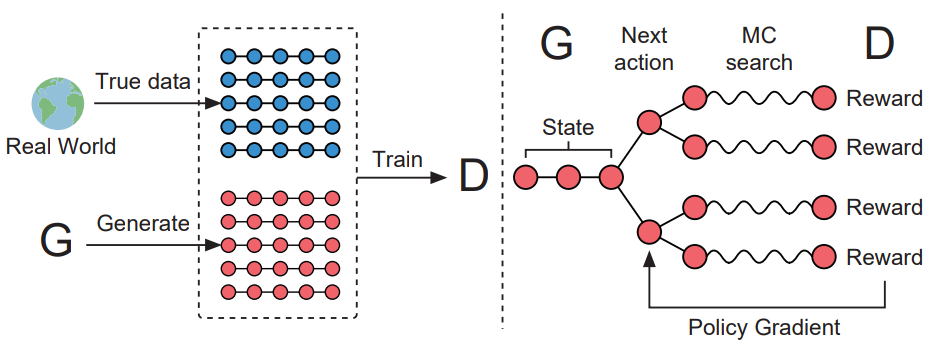
\includegraphics[width=\textwidth]{SeqGAN_Idea.png}
\end{figure}
\end{frame}


\begin{frame}
\frametitle{SeqGAN Algorithm}
\begin{figure}[ht]
  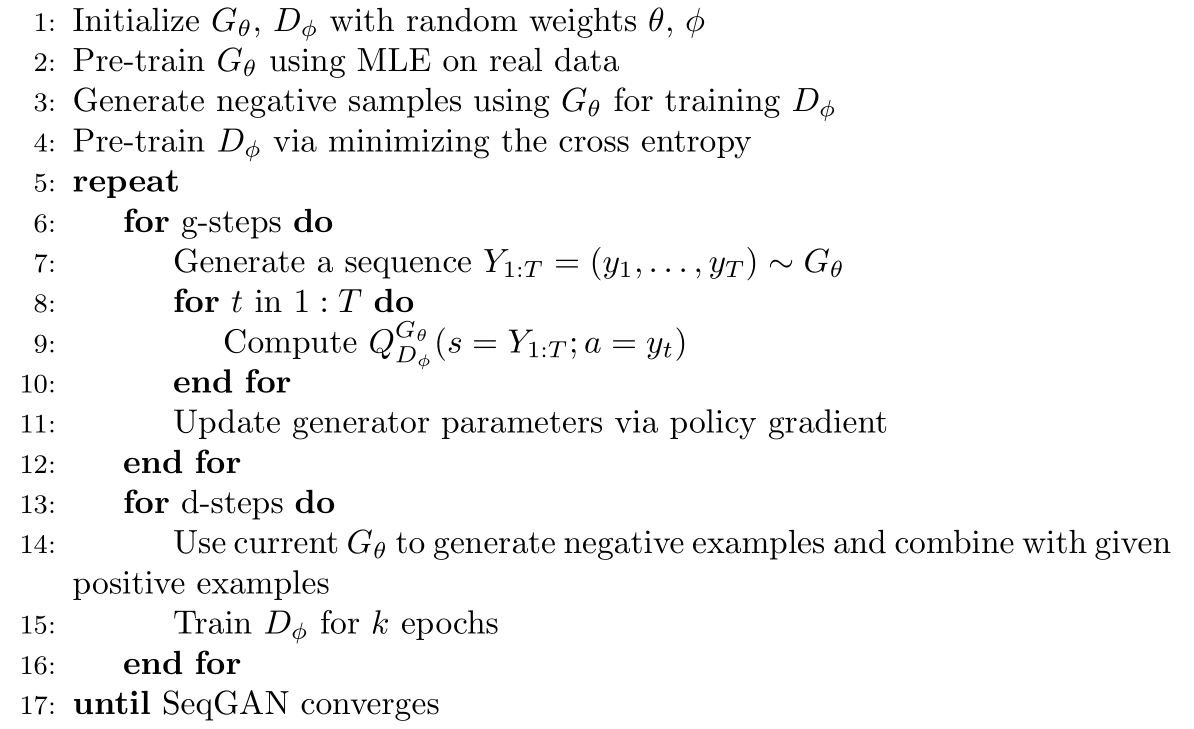
\includegraphics[width=\textwidth]{SeqGAN_Alg.png}
\end{figure}
\end{frame}



%\begin{frame}
%\frametitle{template}
%\begin{figure}[ht]
%  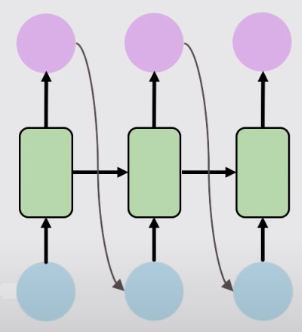
\includegraphics[width=\textwidth]{RNN.png}
%\end{figure}
%\end{frame}

\begin{frame}
\frametitle{LeakGAN}
\begin{figure}[ht]
  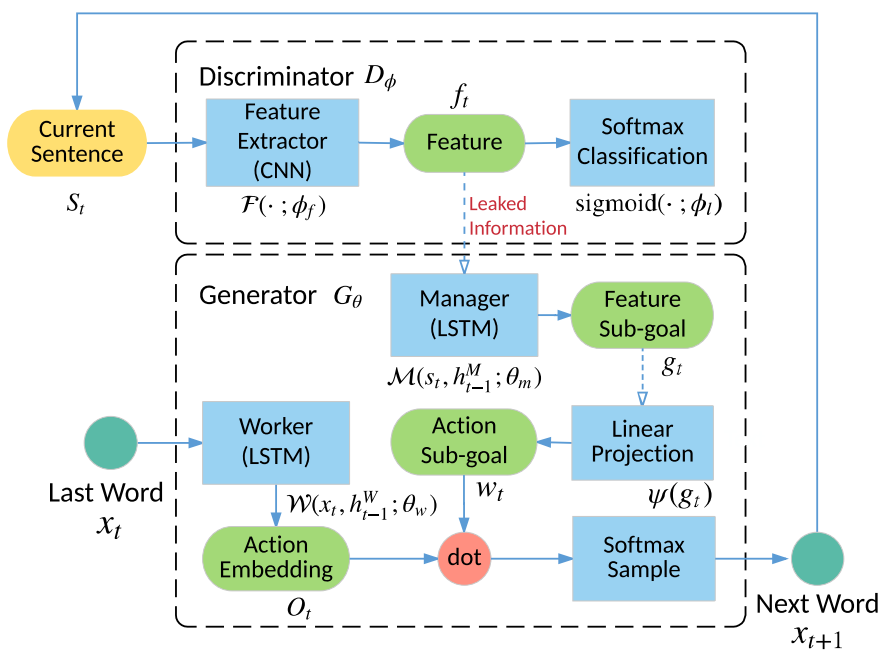
\includegraphics[width=\textwidth]{LeakGAN_Arch.png}
\end{figure}
\end{frame}

\begin{frame}
\frametitle{LeakGAN Algorithm}
\begin{figure}[ht]
  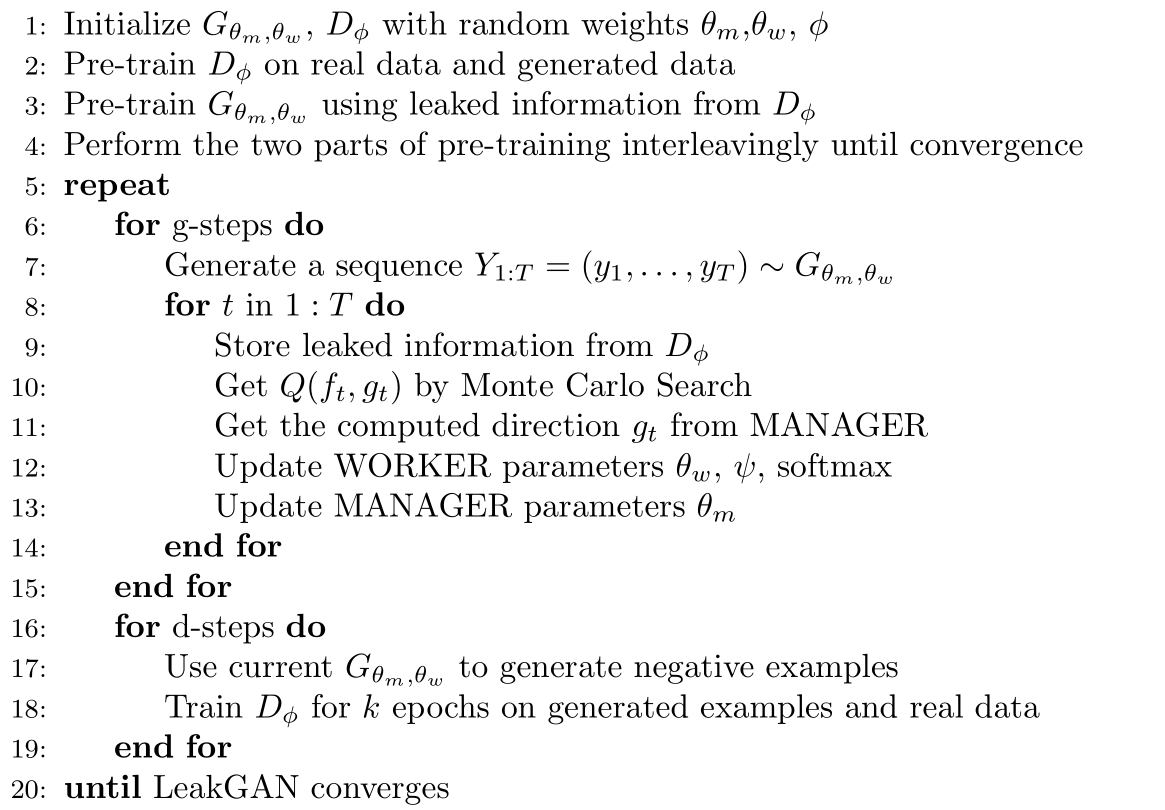
\includegraphics[width=\textwidth]{LeakGAN_Alg.png}
\end{figure}
\end{frame}

\begin{frame}
\frametitle{Avoiding Model Collapse}
\begin{itemize}
  \item Pre-Train
  \item Dropout
  \item Regularization
  \item Interleaved Training
\end{itemize}
\end{frame}

\begin{frame}
\frametitle{Comparison}
\begin{figure}[ht]
  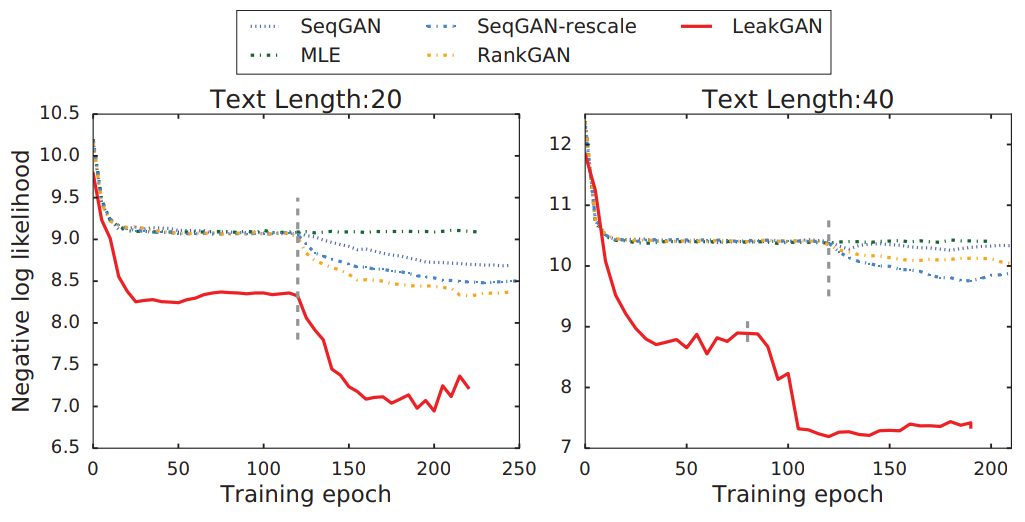
\includegraphics[width=\textwidth]{LeakGAN_vs_SeqGAN.png}
  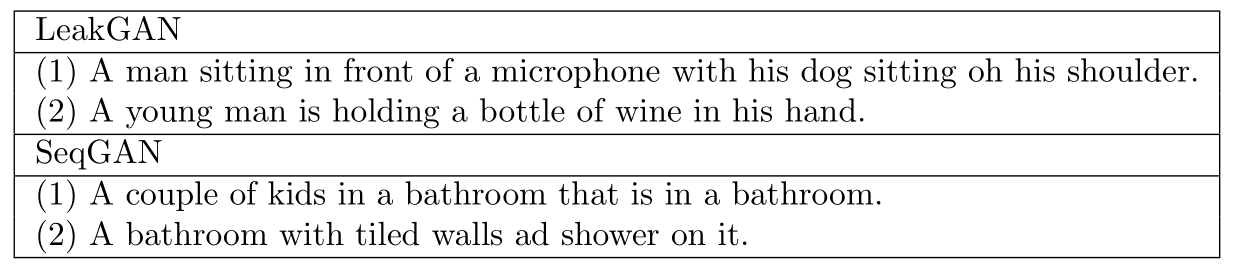
\includegraphics[width=\textwidth]{Gen_seq.png}
\end{figure}
\end{frame}

% AE.png
% 
% VAE.png
% VAE_reparam_trick_backprop.png
% VAE_reparam_trick.png
% 
% GAN.png
% 
% RL_key_concept.png
% Q-Function.png
% 
% Discounted_Total_Reward.png
% Discounted_Total_Reward_Formula.png
% QNN.png
% 
% Policy_Fun.png
% Pol_Grad.png
% 
% SeqGAN_Idea.png
% RNN.png
% 
% LeakGAN_Arch.png
% LeakGAN_vs_SeqGAN.png






\end{document}
